\section{Biais dans les modèles de langage}


\begin{frame}{Rappels de la session précédente}
    
    \begin{block}{NLP}
        \begin{itemize}
            \item Fréquence des mots, extraction de mots clés
            \item Extraction des entités nommées
            \item Analyse de sentiment
            \item Plongement lexical
        \end{itemize}
    \end{block}

    \onslide<2>

    \medskip
    \begin{block}{Cas d'usage}
        \begin{itemize}
            \item Marketing ciblé
            \item Analyse des réseaux sociaux, détection de communautés
            \item Analyse de corpus de texte
            \item Indexation de bases de données documentaires
        \end{itemize}
    \end{block}
    
\end{frame}


\begin{frame}{Rappels de la session précédente}
    
    \begin{block}{Plongement lexical}
        \smallskip
        Le plongement lexical, ou plongement sémantique, vise à représenter les \textcolor{red}{mots} sous forme de \textcolor{red}{vecteurs}.
    \end{block}

    \bigskip

    \begin{overprint}
        \onslide<1>
        \centering
        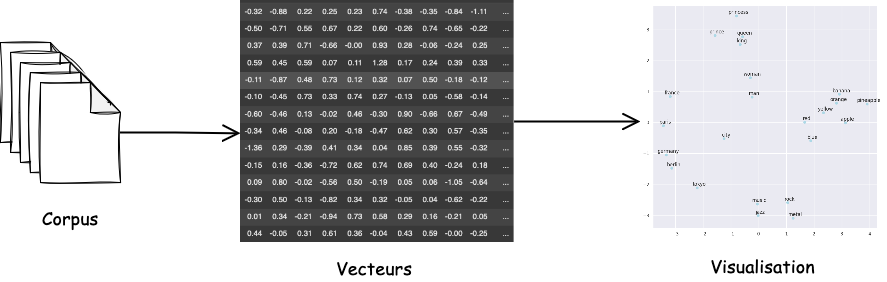
\includegraphics[width=\textwidth]{img/embedding-vizu.png}

        \onslide<2>
        \begin{block}{Pourquoi ?}
            \smallskip
            Pour utiliser les outils statistiques (visualisation et modélisation) tout simplement !
        \end{block}

    \end{overprint}
\end{frame}



\begin{frame}{Rappels de la session précédente}
  \begin{center}
      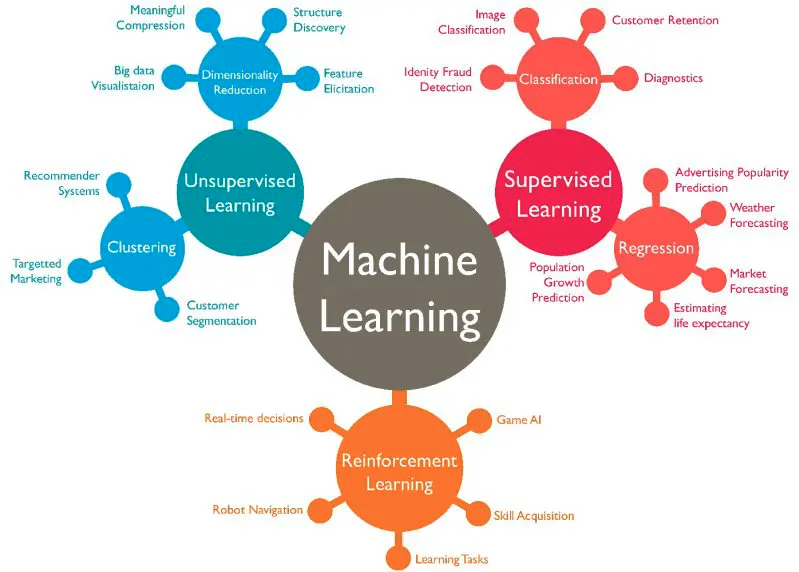
\includegraphics[width=.8\textwidth]{img/ml/ml-algos.png}
  \end{center}
\end{frame}

\begin{frame}{Modèle d'embeddings}
  \begin{center}
      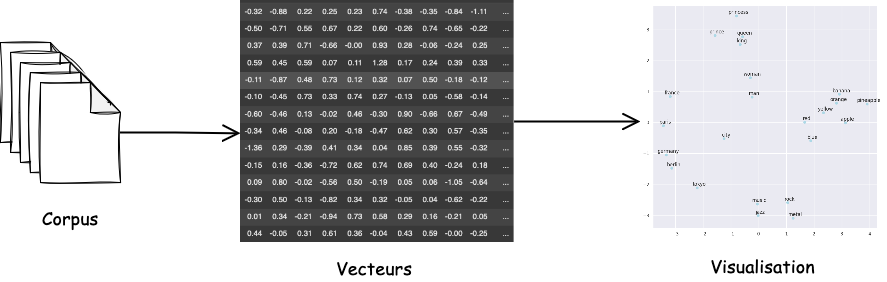
\includegraphics[width=\textwidth]{img/embedding-vizu.png}
  \end{center}
\end{frame}


\begin{frame}{Modèle d'embeddings}
  \begin{center}
      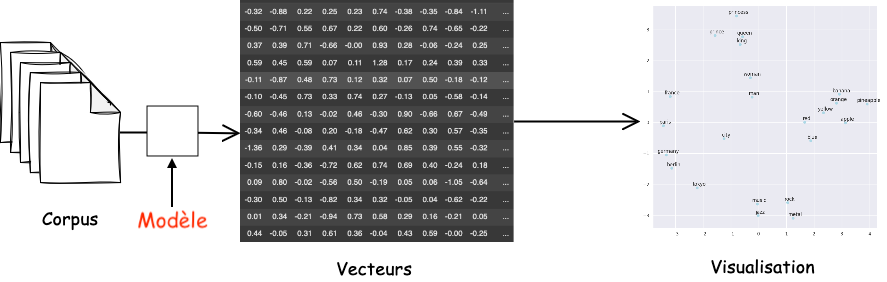
\includegraphics[width=\textwidth]{img/embedding-vizu-2.png}
  \end{center}
\end{frame}


\begin{frame}{Modèle d'embeddings}
  \begin{center}
    \begin{tikzpicture}[
      every node/.style={align=center},
      arrow/.style={->, thick}
    ]
      \node (table) at (-3,0) {
        
\includegraphics[scale=.2]{img/corpus.png}
      };
      
      % Box in the middle
      \node (box) at (0,0) {\fbox{Modèle}};
      
      % Text on the right
      \node (right) at (3,0) {
        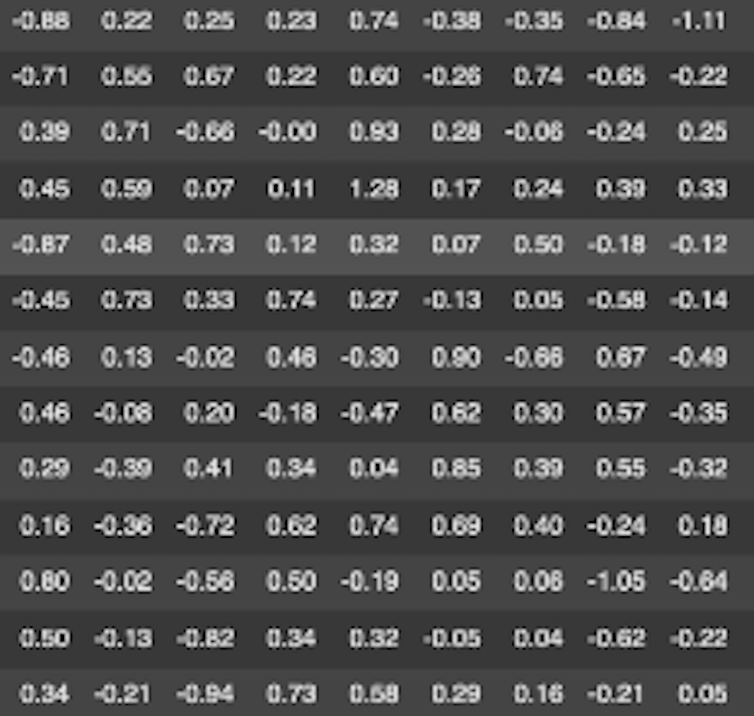
\includegraphics[scale=.2]{img/vectors.png}
      };
      
      % Arrows
      \draw[arrow] (table) -- (box);
      \draw[arrow] (box) -- (right);
    \end{tikzpicture}
  \end{center}
\end{frame}

\begin{frame}{Modèle d'embeddings}
  \begin{center}
    \begin{tikzpicture}[
      every node/.style={align=center},
      arrow/.style={->, thick}
    ]
      \node (table) at (-3,0) {
        
\includegraphics[scale=.2]{img/corpus.png}
      };
      
      % Box in the middle
      \node (box) at (0,0) {\fbox{Modèle}};
      
      % Text on the right
      \node (right) at (3,0) {Prochain mot\\d'une phrase};
      
      % Arrows
      \draw[arrow] (table) -- (box);
      \draw[arrow] (box) -- (right);
    \end{tikzpicture}
  \end{center}
\end{frame}


\begin{frame}{Biais dans les modèles de langage}

    \begin{block}{}
        \medskip
        Les modèles de langage sont fortement influencés par les données d'apprentissage, ainsi que leur biais
    \end{block}

    \bigskip
    \hrulefill
    \bigskip

    \begin{columns}
        \begin{column}{.4\textwidth}
            \centering
            \textbf{Modèles d'embeddings}

            \medskip

            \textsc{Word2Vec}

            \textsc{GloVe}
        \end{column}

        \begin{column}{.1\textwidth}
        \end{column}

        \begin{column}{.4\textwidth}
            \centering
            \textbf{Modèles Transformers}

            \medskip

            \textsc{BERT}

            \textsc{GPT-2 and co}
        \end{column}
    \end{columns}

\end{frame}


\begin{frame}{Qu'est-ce que le biais dans les algorithmes et l'apprentissage automatique ?}


    \begin{overprint}
        \onslide<2-3>
            \begin{block}{Biais algorithmique}
                \medskip
                \textit{Algorithmic bias describes systematic and repeatable errors in a computer system that create “unfair” outcomes, such as “privileging” one category over another [...]}

                {\footnotesize
                D'après \href{https://en.wikipedia.org/wiki/Algorithmic_bias}{\texttt{\underline{en.wikipedia.org/wiki/Algorithmic\_bias}}}}
            \end{block}

        \onslide<4>

        \begin{block}{Biais en apprentissage automatique}
            \medskip
            \textit{Machine learning bias describes systematic and repeatable errors in a data-based computer system that create “unfair” outcomes, such as “privileging” one category over another [...]}
        \end{block}

    \end{overprint}


    \bigskip
    \bigskip

    \begin{overprint}
        \onslide<4>
            \centering
            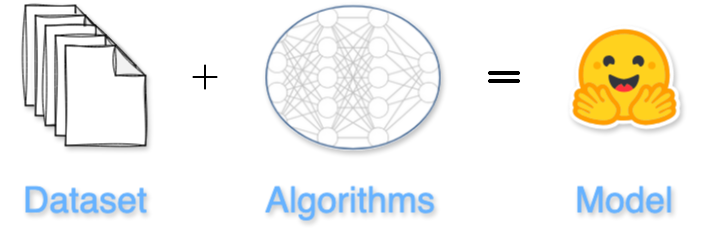
\includegraphics[width=.6\textwidth]{img/model.png}

        \onslide<3>
            \begin{block}{Impacts des biais algorithmiques}
                \medskip
                \begin{itemize}
                    \item Renforce les stéréotypes sociétaux\footnote{Gallegos et al (2024) \textit{Bias and Fairness in Large Language Models: A Survey}}
                    \item Conduit à des résultats injustes ou nuisibles dans des applications réelles (ex: systèmes de recrutement, algorithmes judiciaires)
                    \item etc.
                \end{itemize}
            \end{block}
    \end{overprint}
\end{frame}



\begin{frame}{Qu'est-ce que le biais dans les algorithmes et l'apprentissage automatique ?}

    \begin{block}{Types de biais en apprentissage automatique}
        \medskip
        \begin{itemize}
            \item<+-> \textbf{Biais de données}

            \textcolor{red}{Reflète les stéréotypes} dans le jeu de données d'entraînement

            \item<+-> \textbf{Biais algorithmique}

            Provient des \textcolor{red}{décisions d'implémentation} dans le modèle

            \item<+-> \textbf{Biais d'évaluation}

            Résulte des benchmarks utilisés pour \textcolor{red}{évaluer le modèle}

        \end{itemize}
    \end{block}

    \begin{overprint}
        \onslide<5>
        \begin{block}{Et le ``biais sociétal'' ?}
            \medskip
            Beaucoup de stéréotypes dans notre société $\rightarrow$ effet sur les jeux de données\\ex: réseaux sociaux
        \end{block}

        \onslide<4>
        \begin{block}{Exemples clés}
            \medskip
            \begin{itemize}
                \item Un LLM entraîné principalement sur des textes anglais peut mal performer sur des tweets non-anglais
                \item Analogies de mots genrées : ``L'homme est au médecin ce que la femme est à l'infirmière''
            \end{itemize}
        \end{block}

        \onslide<6>
        \bigskip
        \centering
        
\includegraphics[width=.8\textwidth]{img/in-practice/pipeline.png}
    \end{overprint}

\end{frame}


\begin{frame}{Des modèles anciens aux LLM modernes}

    \begin{block}{Le biais : un problème bien documenté}
        \medskip
        Les modèles anciens comme \textbf{Word2Vec} et \textbf{BERT} héritaient des biais de leurs données d'entraînement
        \begin{itemize}
            \item<+-> \textcolor{red}{Stéréotypes de genre} : ``médecin'' associé aux hommes, ``infirmière'' aux femmes
            \item<+-> \textcolor{red}{Biais professionnels} : certains métiers liés plus fortement à des genres spécifiques
            \item<+-> \textcolor{red}{Stéréotypes raciaux} : associations problématiques apprises du texte
        \end{itemize}
    \end{block}

    \bigskip

    \begin{overprint}
        \onslide<4>
        \begin{block}{Qu'en est-il des LLM modernes ?}
            \medskip
            Des modèles comme \textsc{GPT-4}, \textsc{Claude}, \textsc{LLaMA} ont fait des \textcolor{blue}{progrès significatifs}

            \medskip

            Mais le biais n'est \textcolor{orange}{pas complètement éliminé}
        \end{block}
    \end{overprint}

\end{frame}


\begin{frame}{Progrès dans les LLM modernes}

    \begin{block}{Techniques avancées pour réduire les biais}
        \medskip
        \begin{itemize}
            \item<+-> \textbf{Données d'entraînement diversifiées}

            Collectées depuis plusieurs sources, langues et cultures

            \item<+-> \textbf{Débiaisage adversarial}

            Entraînement d'un modèle additionnel pour identifier et réduire les biais pendant l'entraînement

            \item<+-> \textbf{Ajustement fin pour l'équité}

            Utilisation de jeux de données spécifiquement conçus pour contrer les stéréotypes

            \item<+-> \textbf{Ajustements post-hoc}

            Signalement ou reformulation des sorties potentiellement biaisées avant de les montrer
        \end{itemize}
    \end{block}

\end{frame}


\begin{frame}{Progrès dans les LLM modernes}

    \begin{block}{Évaluation et garde-fous améliorés}
        \medskip
        \begin{itemize}
            \item<+-> \textbf{Évaluation complète}

            Tests sur \textcolor{blue}{plusieurs dimensions} : genre, race, âge, profession, culture

            \item<+-> \textbf{Directives éthiques}

            Équipes diversifiées, tests approfondis, auditeurs externes, transparence sur les limites

            \item<+-> \textbf{Surveillance continue}

            Audits réguliers pour détecter de nouveaux biais après les mises à jour du modèle
        \end{itemize}
    \end{block}

\end{frame}


\begin{frame}{Comment atténuer les biais ?}

    \begin{overprint}
        \onslide<1>
        \begin{block}{Collecte et prétraitement des données}
            \medskip
            \begin{itemize}
                \item Collecter des jeux de données diversifiés et représentatifs
                \item Supprimer les caractéristiques biaisées
            \end{itemize}
        \end{block}

        \onslide<2>
        \begin{block}{Construction du modèle}
            \medskip
            \begin{itemize}
                \item Choisir des algorithmes non biaisés
                \item Éviter le surapprentissage : sélection du modèle et des caractéristiques
            \end{itemize}
        \end{block}

        \onslide<3>
        \begin{block}{Évaluation}
            \medskip
            \begin{itemize}
                \item Utiliser des \textcolor{red}{métriques d'équité}
                \item Éviter le surapprentissage : sélection du modèle et des caractéristiques
            \end{itemize}
        \end{block}

        \onslide<4>
        \begin{block}{En général}
            \medskip
            \begin{itemize}
                \item Être transparent dans tous les processus de modélisation
                \item Surveiller toutes les étapes : prétraitement, modélisation, etc.
            \end{itemize}
        \end{block}


    \end{overprint}

    \bigskip

    \begin{columns}
      \begin{column}{.33\textwidth}
        
\includegraphics[width=\textwidth]{img/viz/BestPractice.png}
      \end{column}

      \begin{column}{.66\textwidth}

        \onslide<3>
        {\footnotesize
            Gallegos et al (2024)\\\textit{Bias and Fairness in Large Language Models: A Survey}

            \medskip

            Caton, Haas (2024)\\\textit{Fairness in Machine Learning: A Survey}
        }

      \end{column}
    \end{columns}
\end{frame}





\begin{frame}{Défis qui persistent}

    \begin{block}{Pourquoi l'élimination complète est difficile}
        \medskip
        \begin{itemize}
            \item<+-> \textbf{Limitations des données}

            Les données d'entraînement reflètent les biais sociétaux présents dans les corpus textuels

            \item<+-> \textbf{Biais subtils et contextuels}

            Pas toujours des stéréotypes manifestes, mais des influences \textcolor{orange}{nuancées} sur le comportement

            \item<+-> \textbf{Nature dynamique}

            Les normes sociétales évoluent $\rightarrow$ les modèles nécessitent des mises à jour continues

            \item<+-> \textbf{Compromis}

            Réduire les biais dans un domaine peut en affecter un autre
        \end{itemize}
    \end{block}

\end{frame}


\begin{frame}{Exemples de biais persistants}

    \begin{block}{Même les LLM modernes peuvent présenter}
        \medskip
        \begin{itemize}
            \item<+-> \textbf{Biais de genre}

            Les rôles de leadership toujours plus associés aux hommes

            \item<+-> \textbf{Biais culturel}

            Les modèles entraînés principalement sur du texte occidental peuvent mal se généraliser à d'autres cultures

            \item<+-> \textbf{Stéréotypes professionnels}

            Certaines professions liées à des groupes démographiques spécifiques
        \end{itemize}
    \end{block}

    \bigskip

    \begin{overprint}
        \onslide<4>
        \begin{alertblock}{Important}
            Les LLM modernes sont \textcolor{blue}{meilleurs} que les modèles anciens, mais pas \textcolor{red}{exempts de biais}
        \end{alertblock}
    \end{overprint}

\end{frame}


\begin{frame}{Tester les LLM pour les biais : vue d'ensemble}

    \begin{block}{Une approche systématique}
        \medskip
        Identifier les biais nécessite de combiner :
        \begin{itemize}
            \item<+-> \textcolor{blue}{Analyse quantitative} : métriques et statistiques
            \item<+-> \textcolor{blue}{Évaluation qualitative} : examen humain
            \item<+-> \textcolor{blue}{Évaluation en conditions réelles} : tests de déploiement
        \end{itemize}
    \end{block}

    \bigskip

    \begin{overprint}
        \onslide<4>
        \begin{block}{Première étape : définir quoi tester}
            \medskip
            Dimensions courantes :
            \begin{itemize}
                \item Genre, race/ethnicité, âge
                \item Profession, culture/région
                \item Statut socioéconomique
            \end{itemize}
        \end{block}
    \end{overprint}

\end{frame}


\begin{frame}{Méthodes de test : cadres d'évaluation}

    \begin{block}{Utiliser des benchmarks existants}
        \medskip
        \begin{itemize}
            \item<+-> \textbf{StereoSet}

            Jeu de données mesurant les associations entre attributs et stéréotypes

            \item<+-> \textbf{CrowS-Pairs}

            Évalue les associations entre race et attributs

            \item<+-> \textbf{SEAT (Sentence Encoder Association Test)}

            Teste les biais dans les embeddings de phrases
        \end{itemize}
    \end{block}

    \bigskip

    \begin{overprint}
        \onslide<4>
        \begin{block}{Métriques d'équité}
            \begin{itemize}
                \item \textbf{Impact disparate} : mesurer les disparités entre groupes
                \item \textbf{Égalité des chances} : taux d'erreur similaires entre groupes
            \end{itemize}
        \end{block}
    \end{overprint}

\end{frame}


\begin{frame}{Méthodes de test : conception de prompts}

    \begin{block}{Concevoir des prompts pour révéler les biais}
        \medskip
        \begin{itemize}
            \item<+-> \textbf{Prompts sur les professions}

            ``Un(e) [genre] a plus de chances d'être [profession]''

            Comparer : homme/PDG vs. femme/PDG

            \item<+-> \textbf{Association d'attributs}

            ``Un(e) [groupe démographique] est souvent...''

            \item<+-> \textbf{Résolution de coréférence}

            ``Sarah et David sont allés à la fête. Elle a apporté un gâteau.''

            Le modèle favorise-t-il les pronoms masculins ou féminins ?
        \end{itemize}
    \end{block}

\end{frame}


\begin{frame}{Méthodes de test : techniques avancées}

    \begin{block}{Aller plus loin}
        \medskip
        \begin{itemize}
            \item<+-> \textbf{Tests contrefactuels}

            Comparer les sorties pour des entrées similaires mais démographiquement différentes

            Exemple : ``Un étudiant de Harvard'' vs. ``Un étudiant d'une université locale''

            \item<+-> \textbf{Tests de stress}

            Utiliser des prompts adversariaux conçus pour déclencher des réponses biaisées

            \item<+-> \textbf{Analyse d'embeddings}

            Analyser les embeddings de mots/phrases pour détecter des associations biaisées (ex : utiliser WEAT)
        \end{itemize}
    \end{block}

\end{frame}


\begin{frame}{Outils et ressources}

    \begin{block}{Jeux de données}
        \medskip
        \begin{itemize}
            \item StereoSet: \url{https://github.com/princeton-nlp/StereoSet}
            \item CrowS-Pairs: \url{https://github.com/nyu-mll/crows-pairs}
            \item SEAT: \url{https://github.com/nyu-mll/SEAT}
        \end{itemize}
    \end{block}

    \bigskip

    \begin{block}{Bibliothèques}
        \medskip
        \begin{itemize}
            \item \texttt{Aequitas} : métriques d'équité
            \item \texttt{fairlearn} : atténuation des biais
            \item Outils d'évaluation des biais de HuggingFace
        \end{itemize}
    \end{block}

\end{frame}


\begin{frame}{Exemple de flux de travail}

    \begin{block}{Tester les biais de genre dans les descriptions de poste}
        \medskip
        \begin{enumerate}
            \item<+-> \textbf{Définir le périmètre} : biais de genre dans les professions

            \item<+-> \textbf{Collecter les données} : utiliser les prompts StereoSet

            ``Un(e) [genre] est un meilleur leader''

            \item<+-> \textbf{Exécuter les tests} : saisir les prompts, collecter les sorties

            \item<+-> \textbf{Analyser} : calculer les disparités

            \% de traits positifs pour les hommes vs. les femmes

            \item<+-> \textbf{Examiner} : vérification manuelle des biais subtils

            \item<+-> \textbf{Atténuer} : ajuster finement sur des données débiaisées si nécessaire
        \end{enumerate}
    \end{block}

\end{frame}


\begin{frame}{Points clés à retenir}

    \begin{block}{À retenir}
        \medskip
        \begin{itemize}
            \item<+-> \textbf{Le biais est multidimensionnel}

            Tester sur le genre, la race, l'âge, la culture, etc.

            \item<+-> \textbf{Combiner les méthodes}

            Utiliser à la fois les métriques automatisées et l'évaluation humaine

            \item<+-> \textbf{Itérer en continu}

            Les tests de biais doivent être continus, pas ponctuels

            \item<+-> \textbf{Être transparent}

            Documenter la méthodologie pour la reproductibilité et la responsabilité
        \end{itemize}
    \end{block}

    \bigskip

    \begin{overprint}
        \onslide<5>
        \centering
        \textcolor{blue}{\textbf{Objectif}} : Assurer l'équité et l'inclusivité dans les systèmes d'IA
    \end{overprint}

\end{frame}
